\documentclass{article}
\usepackage{graphicx,wrapfig}
\usepackage[a4paper, total={6in, 10in}]{geometry}
\usepackage{amsmath}
\usepackage{amssymb,amsthm}
\usepackage{tikz}
\usepackage{inconsolata}

\usepackage{color}

\definecolor{pblue}{rgb}{0.13,0.13,1}
\definecolor{pgreen}{rgb}{0,0.5,0}
\definecolor{pred}{rgb}{0.9,0,0}
\definecolor{pgrey}{rgb}{0.46,0.45,0.48}

\usepackage{listings}
\lstset{language=Java,
  showspaces=false,
  showtabs=false,
  breaklines=true,
  showstringspaces=false,
  breakatwhitespace=true,
  commentstyle=\color{pgreen},
  numberstyle=\tiny,
  keywordstyle=\color{pblue},
  stringstyle=\color{pred},
  basicstyle=\ttfamily\footnotesize,
  numbers=left,                    
  numbersep=5pt,  
  moredelim=[il][\textcolor{pgrey}]{$ $},
  moredelim=[is][\textcolor{pgrey}]{\%\%}{\%\%}
}


\usepackage[
backend=biber,
style=apa,
]{biblatex}
\addbibresource{main.bib} %Imports


\renewcommand{\contentsname}{Indholdsfortegnelse}

\title{Studieretnings Case - Fraktaler}
\author{Victor Østergaard Nielsen, 2di}
\date{Maj 2024}

\setcounter{figure}{0}
\renewcommand{\figurename}{Figur}
\renewcommand{\thefigure}{\arabic{figure}}

\begin{document}

\maketitle

\section*{}
\begin{figure}[!h]
    \centering
    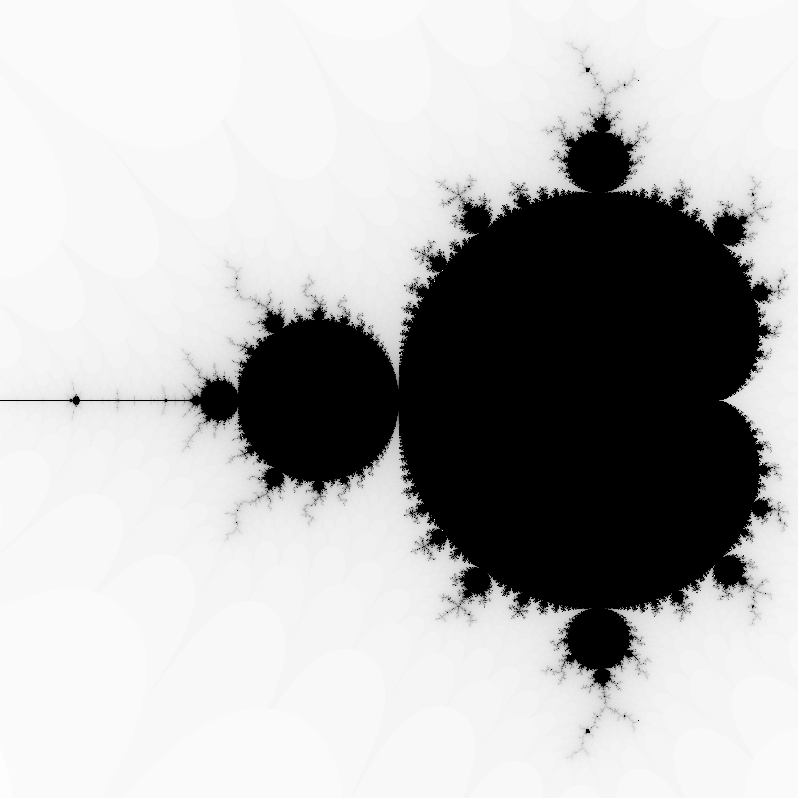
\includegraphics[width=0.7\linewidth]{fractal1.png}
    \caption{Mandelbrotmængden}
    \label{mandelbrotmængden}
\end{figure}

\newpage

\section*{Tro- og loveerklæring}
Jeg bekræfter herved med min underskrift, at denne studieretnings case er udarbejdet af mig. Jeg har ikke anvendt tidligere bedømt arbejde uden henvisning hertil, og opgaven er udfærdiget uden anvendelse af uretmæssig hjælp og uden brug af hjælpemidler, der ikke har været tilladt i forbindelse med projektet.\\\\\\
%
Victor Østergaard Nielsen d. \hrulefill\\\\\\
%
Underskrift: \hrulefill\\

\newpage

\section*{Opgavens Problemstilling: Matematik værktøj til hjælp af forståelse af fraktaler}
\textbf{Hvordan kan fraktaler anvendes i programmering og matematik, og hvordan kan forståelsen af disse komplekse systemer øges ved hjælp af visuelle værktøjer?}\\\\
Redegørelse
\begin{itemize}
    \item Hvordan defineres fraktaler matematisk, og hvordan kan de visualiseres i en programmeringssammenhæng?
    \item Definer komplekse tal og deres sammenhæng med fraktaler.
    \item Teori omhandlende det objekt orienteret paradigme
\end{itemize}
Analyse
\begin{itemize}
    \item Hvilke metoder anvendes typisk til visualisering af fraktaler i programmeringssprog og hvordan kan processen optimeres?
    \item Hvordan bygges en oop brugerflade
\end{itemize}
Vurdering og diskussion
\begin{itemize}
    \item Afgør om hvorvidt programmet tilnærmer fraktalernes formler tilstrækkeligt
    \item Vurder og diskuter desuden på programmet og resultaterne
\end{itemize}
Perspektivering
\begin{itemize}
    \item kystlinje
\end{itemize}

\newpage
\tableofcontents
\newpage

\section{Hvad er fraktaler}
For at kunne besvare problemformuleringen præcist, er en klar definition af en fraktal relevant. Selv om kilderne er lidt uenige, kan man groft sagt definere en fraktal således: En fraktal er en særlig type geometrisk form eller mønster, som besidder mindst én af følgende karakteristika: For det første kan den indeholde detaljer, uanset hvor meget man zoomer ind. Med andre ord forbliver strukturen kompleks på selv de mindste skalaer. For det andet er fraktaler så uregelmæssige og kaotiske i deres natur, at de ikke lader sig beskrive præcist med de klassiske geometriske begreber og metoder. Deres form er for kompliceret til de traditionelle geometriske rammer. I denne opgave vil der primært være fokus på den første slags.\parencite{vestergaard}\\
\subsection{Sierpinski-trekanten}
\begin{wrapfigure}{r}{6cm}
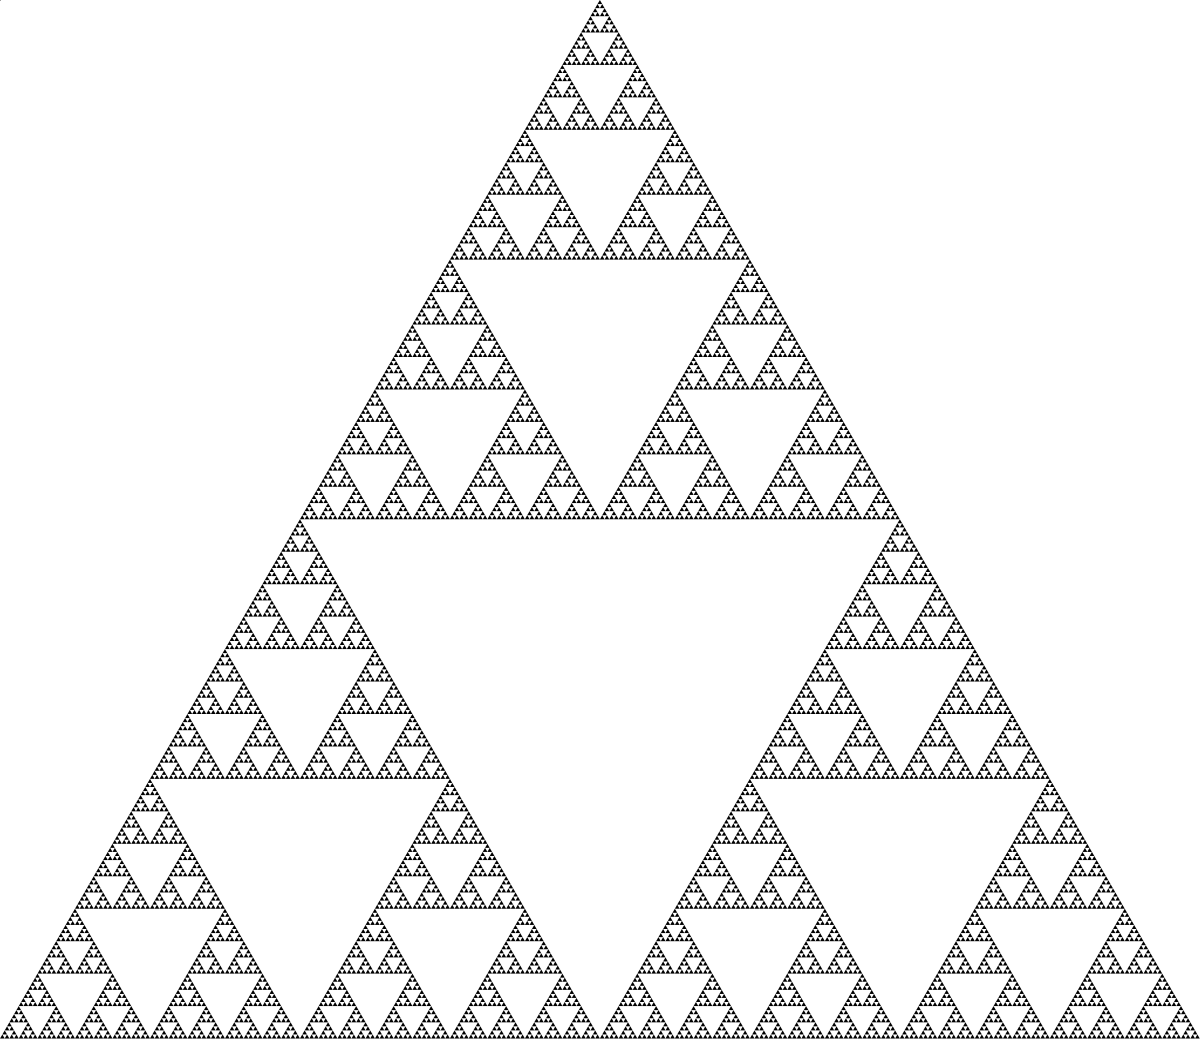
\includegraphics[width=6cm]{Sierpinski-trekanten}
\caption{Sierpinski-trekanten, iteration $n>8$, fra: \parencite{Stanislaus_2013} }\label{wrap-fig:1}
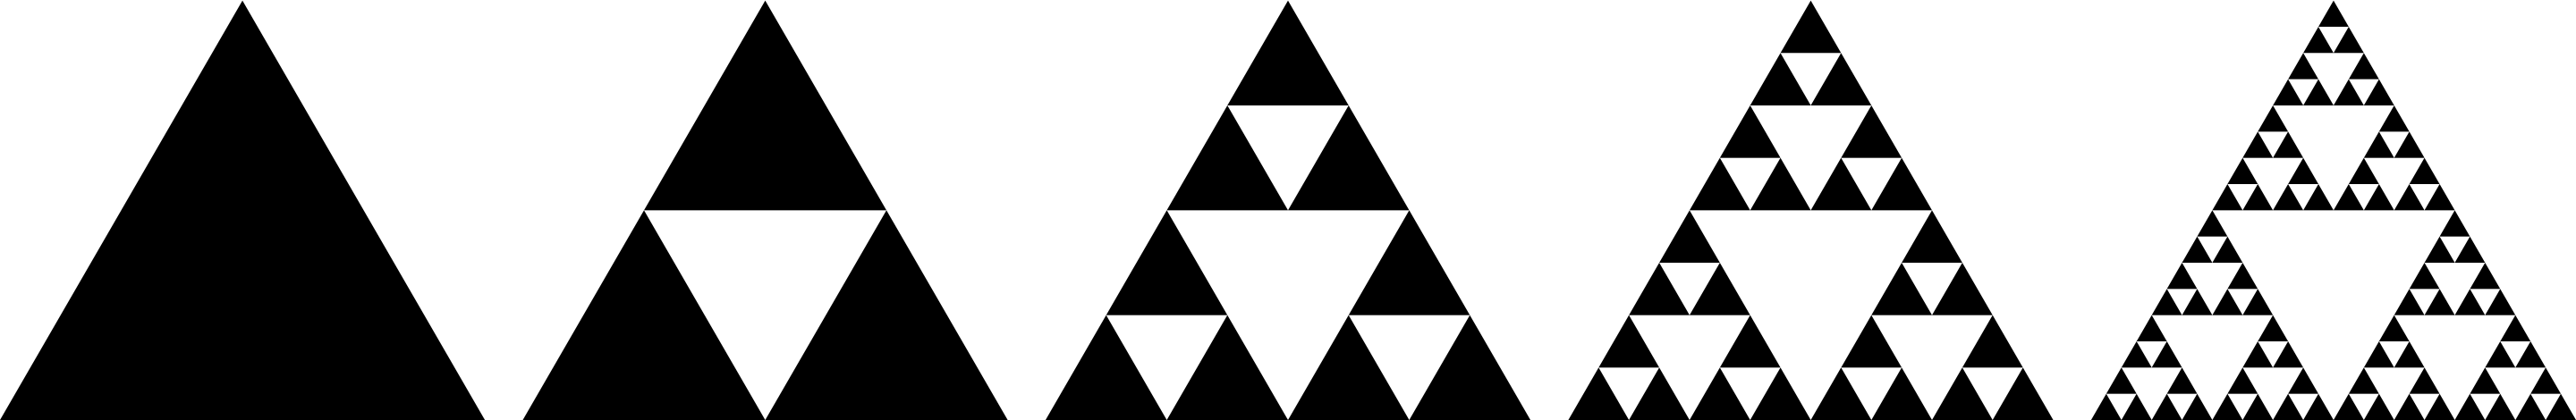
\includegraphics[width=6cm]{Sierpinski_triangle_evolution.png}
\caption{Sierpinski-trekanten, iteration $n=0..4$, fra: \parencite{Saperaud_2006} }\label{wrap-fig:2}
\end{wrapfigure}
Iblandt disse særlige geometriske former og mønstre af uendelig detalje er Sierpinski-trekanten en af de mest velkendte. For at skabe Sierpinski-trekanten skal denne algoritme følges punktligt: Antag en udfyldt ligesidet trekant. Nu forbindes hver af sidernes midtpunkter sammen, hvorefter denne trekant trækkes fra den forrige. Den resulterende figur, som består af 3 ligesidede trekanter, der er ligedannet med starttrekanten, er den første iteration af Sierpinski-trekanten. Hvis $n$ er lig med iterationen, så er $n=1$. For at skabe næste iteration $n=2$ skal samme proces gentages for de 3 mindre trekanter. Denne proces kan ses på Figur \ref{wrap-fig:2} For at opnå Sierpinski-trekanten skal $n=\infty$, alt under $n=\infty$ er blot en tilnærmelse. Antag nu en Sierpinski-trekant, del figuren i 3 dele, forkast 2 af delene, skalér den sidste med en faktor på 2, den resulterende figur vil være lig med den oprindelige Sierpinski-trekant. Den opfylder derfor første kriterie i definitionen heraf og kan derfor betegnes som en fraktal. Sierpinski-trekanten er et eksempel på en fraktal, der viser en unik egenskab. Selvom dens kompleksitet stiger, nærmer dens areal sig $0$, mens dens omkreds stiger mod $\infty$. Dette fænomen udstiller en interessant kontrast mellem dens faldene areal, og dens stigende omkreds. Således er Sierpinski-trekanten eksempel på en slags geometrisk paradoks.\\
\subsection{Koch’s kurve}
\begin{wrapfigure}{r}{6cm}
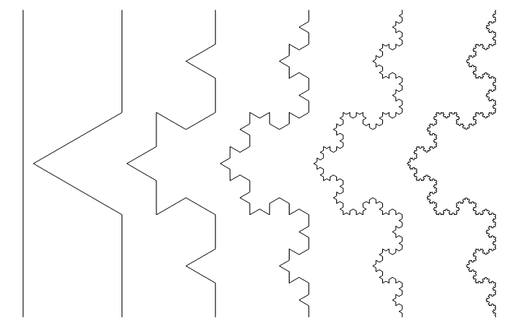
\includegraphics[width=6cm]{kochkurve}
\caption{Koch’s kurve, $n=0..5$}\label{wrap-fig:3}
\end{wrapfigure} 
Koch’s kurve er et andet eksemplar på en selvsimilær figur. Kurven blev først betragtet af den svenske matematiker Niels Fabian Helge von Koch (H. von Koch) i begyndelsen af 1900-tallet. Kurven dannes ved følgende fremgangsmåde: Start med et linjestykke, fjern den midterste tredjedel, og indsæt to linjestykker i stedet, så der dannes en spids med en vinkel på 60 grader, som vist i tegningen til højre. Gentag derefter processen for hver af de fire resulterende linjestykker i den nye figur, ved at erstatte den midterste tredjedel med en spids. Dette resulterer i den tredje figur set til højre. Processen fortsættes gentagne gange. igen siges det at alt under $n=\infty$ er blot en tilnærmelse, hvis $n$ er antallet af iterationer.
\newpage
\subsection{Definition af dimension}
De fleste mennesker støder på begrebet dimensioner i deres hverdag. Udtrykket bliver ofte brugt når man beskriver et objekts udstrækning. For eksempel når man spørger: "Hvad er dimensionerne på kassen?" Her refererer man til bordets længde, højde og bredde. Et andet eksempel er når man taler om "3D-film". Her opfatter man dybden i billedet udover det flade billede. Man siger, at en linje har én dimension (kun længde). En flad firkant har to dimensioner (længde og bredde). Og endelig har en massiv kasse tre dimensioner (længde, bredde og højde). For at kunne beskrive fraktaler skal forståelsen af dimensioner udvides. De selvsimilære fraktaler har den særlige egenskab, at de er sammensat af mindre dele, som hver især ligner den samlede fraktal, bare i mindre skala. Et godt eksempel er Koch's kurve, som illustreret i figur \ref{wrap-fig:3} i forrige afsnit. kurvens mindre grene ligner den overordnede snefnug, bare i mindre format. Denne egenskab ved selvsimilære fraktaler gør, at deres dimension ikke nødvendigvis er et helt tal som 1, 2 eller 3. I stedet kan deres dimension være et ikke-helt decimaltal, som giver et mere nøjagtigt mål for deres kompleksitet.
\subsubsection{Hausdorff dimension}
Lad os antage, at $n$ er antallet af de formindskede kopier, som fraktalen består af, og lad $s$ være faktoren, man skal gange de formindskede kopier med for at genskabe den fulde fraktal.
Angående $s$, så refererer dette til den lineære forstørrelse. Med andre ord er $s$ forholdet mellem længden af den samlede fraktal og længden af de enkelte formindskede kopier. $s$ kaldes skaleringsfaktoren. Dimensionen for en selvsimilær fraktal er det tal $d$, som opfylder: $$n=s^d$$
Denne definition af dimension kaldes også for \textit{Hausdorff dimension} 
\subsubsection{Minkowski–Bouligand dimension}
\begin{wrapfigure}{r}{4cm}
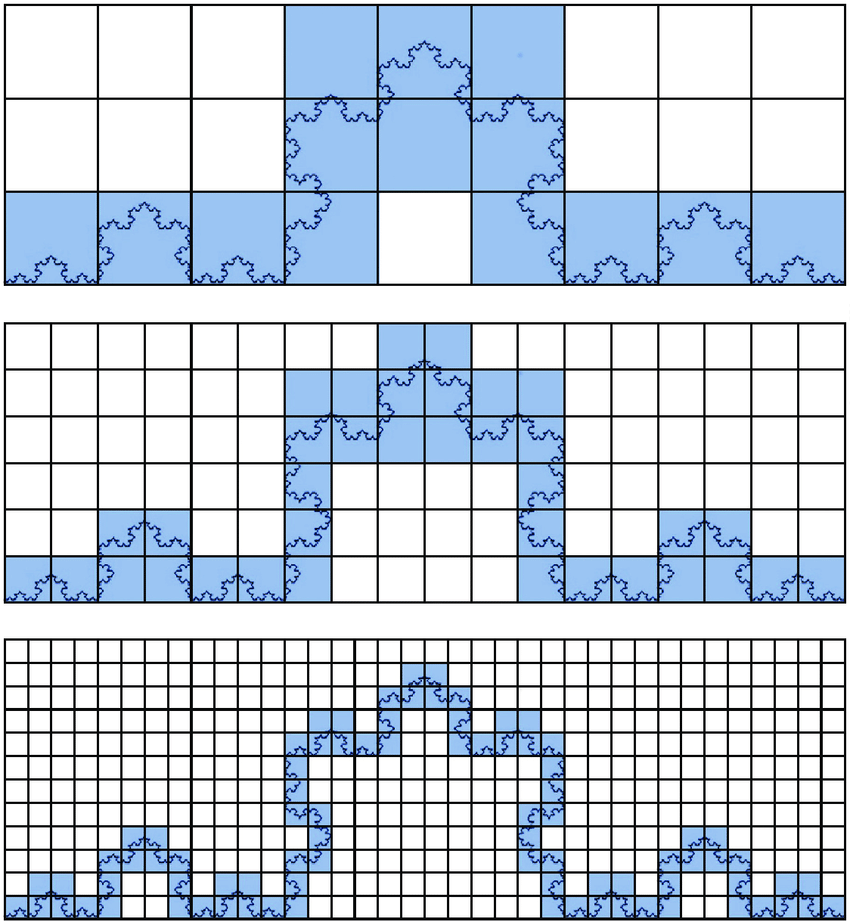
\includegraphics[width=4cm]{boxcount.png}
\caption{Illustration af box-counting på Koch's kurve, fra: \parencite{inbook}}\label{wrap-fig:300}
\end{wrapfigure} 
Hausdorff dimension er kun gældenende for selvsimilære figure idet de her den særlige egenskab, at de er sammensat af mindre dele, som hver især ligner den samlede figur. Minkowski-Bouligand dimensionen, også kendt som box-counting dimensionen, er en måde at kvantificere fraktale strukturer på. Den beregner dimensionen $D$ af et sæt ved at tælle antallet $\text{N}(\epsilon)$ af gitterceller (bokse) af given størrelse $\epsilon$, der indeholder dele af sættet, hvor $D$ defineres som: $$D = \lim_{\epsilon\to0} \frac{\log(\text{N}(\epsilon)}{\log(\frac{1}{\epsilon})}$$
Denne definition dimension tager højde for både selvsimilaritet og ikke selvsimilære figure. Som set på figuren til højre er denne metode kun relevant for kanten af fraktalen, det er en en slags måde at beskrive at der fortsat vil være detalje uanset hvormeget man zoomer ind. \parencite{vestergaard}

\newpage
\section{Matematiske fraktaler}
Før der kan arbejdes med matematiske fraktaler, er en basal viden indenfor komplekse tal såvel som det komplekse plan nødvendig.
\subsection{Komplekse tal}
Komplekse tal ($\mathbb{C}$) betragtes som en udvidelse af de reelle tal ($\mathbb{R}$) og er bestående af to dele:
$$
z=a+b\cdot i,\quad a\in \mathbb {R} ,\;b\in \mathbb {R}
$$
Her er $a$ den reelle del og $b\cdot i$ er den imaginære del. Den imaginære del repræsenteres typisk ved bogstavet $i$, som er defineret som kvadratroden af et negativt tal. det vil sige at: 
$$
i^2=-1
$$
Da det ikke er vigtigt for problemformuleringen hvorfor dette giver mening vil denne del undlades. Ligesom de reelle tal kan man ligeledes udføre addition, subtraktion og multiplikation samt andre operationer på komplekse tal:\\\\
Givet: $z_1=a+bi$ og $z_2=c+di$
\begin{align*} 
     z_1+z_2&=(a+bi)+(c+di)=a+bi+c+di=(a+c)+(b+d)i\\
     z_1-z_2&=(a+bi)-(c+di)=(a-c)+(b-d)i\\
z_1\cdot z_2&=(ac - bd) + (ad + bc)i
\end{align*}
Addition, subtraktion er lige ud af landevejen. Multiplikation kan virke lidt kryptisk, men det virker hvis man multiplicere hver del af det første komplekse tal med hver del af det andet komplekse talsiden og husker at $i^2=-1$ \parencite{Cuemath}
\subsection{Det komplekse plan}
\begin{wrapfigure}{r}{6cm}
\resizebox{6cm}{6cm}{ % Resize the tikzpicture to 6cm width and height
    \begin{tikzpicture}
        \begin{scope}[thick,font=\scriptsize]
        
        \draw [->] (-4,0) -- (4,0) node [above left] {$\Re\{z\}$};
        \draw [->] (0,-4) -- (0,4) node [below right] {$\Im\{z\}$};
        
        \foreach \n in {-3,...,-1,1,2,...,3}{%
            \draw (\n,-3pt) -- (\n,3pt) node [above] {$\n$};
            \draw (-3pt,\n) -- (3pt,\n) node [right] {$\n i$};}
            
        \draw [thick, color=red] (0,0) -- (2,3);
        \draw [color=blue, fill=blue] (2,3) circle(0.05);
        \node [color=black] at (3,3) {$2+3i$};
        
        \end{scope}
    \end{tikzpicture}
}
\caption{$z=2+3i$ i Argand-diagram}\label{wrap-fig:5}
\end{wrapfigure} 
Den traditionelle måde at beskrive tal er en linje, lad os kalde denne linje for den \textit{reelle linje}. På denne linje findes alle de naturlige tal ($\mathbb{N}$), alle hele tal ($\mathbb{Z}$), alle Rationelle tal ($\mathbb{Q}$) og alle de Reelle tal ($\mathbb{R}$). Men denne tallinje kan ikke beskrive de komplekse tal ($\mathbb{C}$), der er derfor brug for et nyt system til at indeholde de komplekse tal. Antag et koordinatsystem hvor $x$-aksen er den \textit{reelle linje}, og hvor $y$-aksen er den imaginære akse, beskrevet ved den imaginære del af de komplekse tal. Da der ikke er tale om hverken koordinater, eller $x$ og $y$-akser kan denne talemåde erstattes med hhv. \textit{det komplekse plan} den \textit{reelle akse} og den \textit{imaginære akse}. Det komplekse plan er også tiltalt som et Argand-diagram, efter den schweiziske matematiker Jean-Robert Argand, der i 1806 offentliggjorde hans idé om netop denne geometriske fortolkning af komplekse tal. til højre ses det komplekse tal $z=2+3i$ på et Argand-diagram. Når de komplekse tal vises grafisk, giver det bedre mening hvordan addition, subtraktion og multiplikation virker.
\newpage
\subsection{Mandelbrotmængden}
\begin{wrapfigure}{r}{6cm}
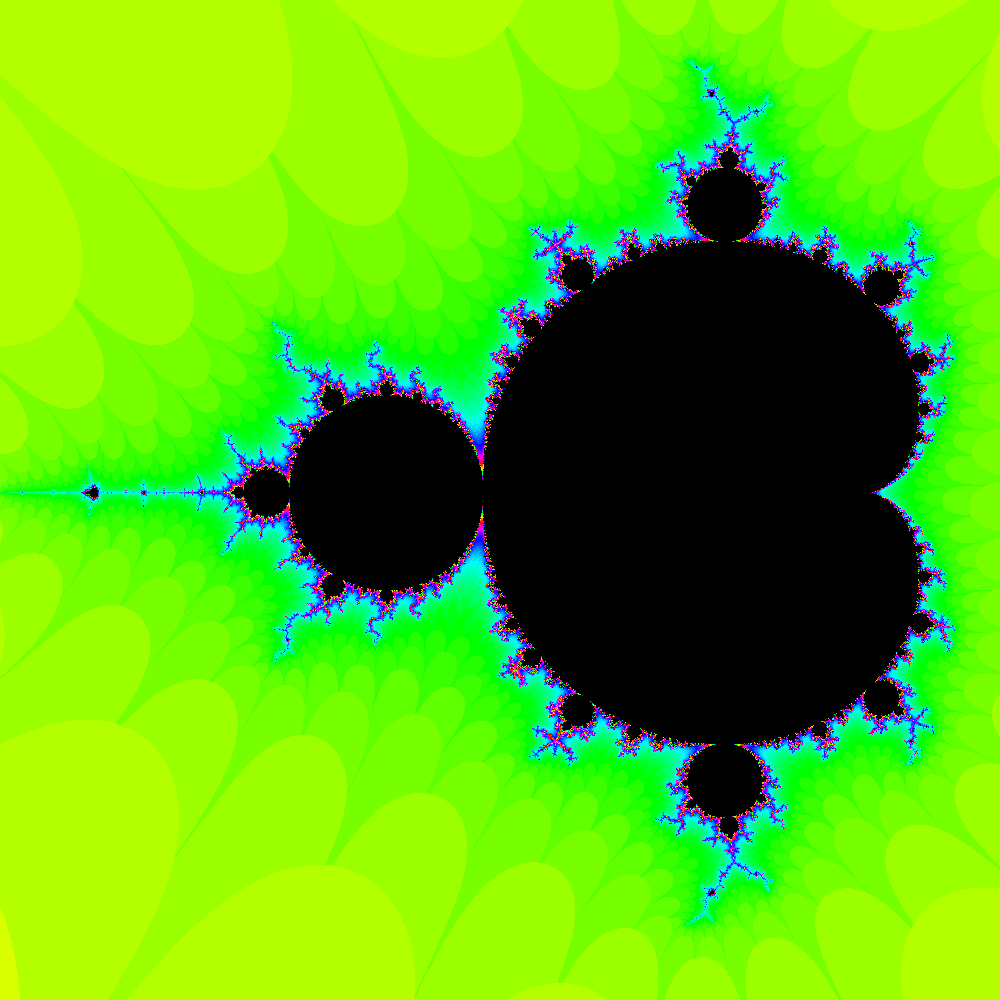
\includegraphics[width=6cm]{madelbrotcolor.png}
\caption{Mandelbrotmængden, $n=100$}\label{wrap-fig:6}
\end{wrapfigure} 
Med en grundforståelse indenfor komplekse tal og det komplekse plan kan mandelbrotmængden nu introduceres. Mandelbrotmængden er givet ved følgende rekursive ligning:
$$
z_{n+1}=z_n^2+c
$$
I Mandelbrotmængden er \( c \) en kompleks konstant. Den repræsenterer punktet på det komplekse plan, som du tester for medlemskab i Mandelbrotmængden. Mandelbrotmængden er en mængde af komplekse tal \( c \), hvor iterationen \( z_{n+1} = z_{n}^2 + c \) divergerer, når den itereres fra \( z_0 = 0 \). Med andre ord, hvis absolutværdien af \( z_{n} \) forbliver begrænset, når \( n \) nærmer sig uendelig, så betragtes \( c \) som værende i Mandelbrotmængden. Hvis absolutværdien af \( z_{n} \) derimod vokser uden grænse, er \( c \) ikke i Mandelbrotmængden. Denne relativt simple ligning viser sig at have overraskende stor kompleksitet og en verden af unikke fraktale mønstre. Billeder af Mandelbrot-mængden, som set til højre, er meget berømte inden for matematikken. \parencite{Videnskab_2023}
\section{Det objekt orienteret paradigme}
\subsection{Indkapsling}
Indkapsling er et princip inden for objektorienteret programmering (OOP), der betyder, at man skjuler objektets interne implementering og tilstand fra omverdenen. Dette opnås ved at begrænse direkte adgang til objektets felter (data) og metoder (funktioner). I stedet eksponeres et veldefineret grænseflade, der kontrollerer, hvordan data kan tilgås og ændres. På denne måde beskyttes objektets integritet og stabilitet. \parencite{Scoutapm_2021} I Java er dette opnået ved brug at \textit{access modifiers}. I Java findes der 3 typer: \texttt{public}, \texttt{private} og \texttt{protected}. Herunder ses forskellene:
\begin{table}[!h]
    \centering
    \begin{tabular}{rl}
        \texttt{public} & Adgang til indholdet for alle klasser\\
        \texttt{private} & Adgang til indholdet er kun mulig i den erklærede klasse\\
        \texttt{protected} & Adgang til indholdet i den samme klasse og i alle underklasser\\
    \end{tabular}
    \label{tab:my_label}
\end{table}\\
Da de interne variabler skal ifølge princippet holdes \texttt{private} eller \texttt{protected}, men hvis disse variabler skal eksponeres, skal det ske gennem såkaldte \textit{getters} og \textit{setters}. Herunder ses en simpel klasses hvor dette princip er inkorporeret:
\lstinputlisting[language=Java]{indkapsling.java}
Mens der i dette eksempel er fri adgang til variablen \texttt{CPR} gennem de defineret \textit{getters} og \textit{setters}, vil der let kunne pålægges regler for, hvem der kan ændre variablen eller hvornår det kan ske. \texttt{protected} er kun relevant hvis en klasse har underklasser.
\newpage
\subsection{Nedarvning}
Nedarvning er et andet meget vigtigt princip indenfor objektorienteret programmering (OOP). Nedarvning i objektorienteret programmering er en slags mekanisme, hvor en klasse kan arve egenskaber og metoder fra en anden klasse. Den nye klasse, der arver, kaldes en underklasse eller en \textit{child}, mens klassen, der bliver arvet fra, kaldes en superklasse eller en \textit{parrent}. Underklassen kan tilgå alle de \texttt{public} og \texttt{protected} variabler og metoder fra superklassen, men kan også tilføje sin egen funktionalitet. Ved at overskrive funktionalitet eller bygge nye funktioner. herunder ses et kort eksempel hvor en nedarvet klasse overskrive en metode:
\lstinputlisting[language=Java]{nedarvning.java}
Her overskrives \texttt{lavLyd()} metoden for at gide hunden en unik lyd, bemærk at underklassen arver \texttt{navn} værdien fra superklassen.
\subsection{SOLID}
SOLID er et velkendt akronym for fem principper for god objektorienteret design, det vil primært arbejdes med de første 2 principper, men de er alle præsenteret herunder for overblikkets skyld:
\begin{itemize}
    \item[S -] Single Responsibility Principle: En klasse bør have ét, velafgrænset ansvar
    \item[O -] Open/Closed Principle: Softwareenheder bør være åbne for udvidelse, men lukkede for modifikation. 
    \item[L -] Liskov Substitution Principle: Underklasser skal kunne erstatte deres overklasser.
    \item[I -] Interface Segregation Principle: Bedre at have mange specifikke interfaces end én generel.
    \item[D -] Dependency Inversion Principle: Moduler på højere niveauer bør ikke afhænge af moduler på lavere niveauer. Begge bør afhænge af abstraktioner.
\end{itemize}
\subsubsection{Single Responsibility Principle}
Single Responsibility Principle siger, at en klasse bør have ét, velafgrænset ansvar. En klasse med mere end et ansvar bliver sværere at forstå, ændre og teste. F.eks. skal \texttt{Hund} kassen ikke have indflydelse/ansvar over \texttt{Menneske} klassen.
\subsubsection{Open/Closed Principle}
Open/Closed Principle siger, at softwareenheder (klasser) bør være åbne for udvidelse, men lukkede for modifikation. Det vil sige, at man bør kunne tilføje ny funktionalitet uden at ændre eksisterende kode. Dette er typisk gjort ved at designe med abstrakte basisklasser og bruge arv og komposition. Og dermed have \textit{søsterklasser}, altså mange klasser som arver fra den samme superklasse.
\section{Visualisering af mandelbrotmængden}
I programmet vil der primært tages udgangspunkt i mandelbrotmængden og hvordan den oversættes til kode, programmerings sproget som vil bruges til fremstilling er Java 21.
% (til relevante dele at udviklingsprocessen vil den være links til min hjemmeside, hvor man kan køre koden i browseren, disse kodestykker er skrævet i Processing 3 og kompileret til P5.js).
\subsection{Oversættelse af: $z_{n+1}=x_n^2+c$ til Java}
Da ligningen er rekursiv, ville et \texttt{while}-loop nok være et godt sted at starte:
\begin{lstlisting}[language=Java]
int n = 0;
while(n < i) {
    n++;
}
\end{lstlisting}
Hvor \texttt{n} er den nuværende iteration og \texttt{i} er det maksimale antal tilladte antal iterationer. Lad os nu inddrage det komplekse tal $c$ som \texttt{ca} og \texttt{ca}, refererende til hhv. den reelle del og den imaginære del. Da $c$ var lig det komplekse tal vi ønsker at undersøge, vil hhv. \texttt{a} og \texttt{b} holde hver del af dette komplekse tal mens der itereres over \texttt{while}-loopet:
\begin{lstlisting}[language=Java]
double a = dmap((double) x, 0D, (double) img.width, (double) (-2.5 / z + ox), (double) (2.5 / z + ox));
double b = dmap((double) y, 0D, (double) img.height, (double) (-2.5 / z + oy), (double) (2.5 / z + oy));
double ca = a + cao;
double cb = b + cbo;
int n = 0;
while(n < i) {
    n++;
}
\end{lstlisting}
\textit{\texttt{dmap()} er bare en \texttt{map()} funktion til typen \texttt{double}}\\
Her defineres \texttt{a} og \texttt{b} som hjørnet at det vindue vi kigger i, vinduet er defineret med en zoom variabel {\texttt{z}} og et x og y offset (\texttt{ox} og \texttt{oy}). \texttt{2.5} er igen bare et fastlagt offset for at starte det rigtige sted. Nu kan den næste iteration udregnes. $z_{n+1}$ er givet i koden som \texttt{aa} og \texttt{bb} stående for hver det af det komplekse tal, \texttt{cao} og \texttt{cbo} er igen bare offsets, disse er normalt sat til 0:
\begin{lstlisting}[language=Java]
...
while(n < i) {
    double aa = a * a - b * b;
    double bb = 2 * a * b;
    a = aa + ca;
    b = bb + cb;
    n++;
}
\end{lstlisting}
\texttt{aa = a * a - b * b} og \texttt{bb = 2 * a * b} er givet ud fra formlen $(a + bi)^2 = a^2 - b^2 + 2abi$. Derfor må $z_{n+1}$ være lig: $(a, b) = (aa + ca, bb + cb)$ som implementeret i kode i linje 5-6 herover. hvis $a+b$ eksploderer i størrelse er tallet ikke en den at mandelbrotmængden, dette kan også tilføjes til koden:
\begin{lstlisting}[language=Java]
...
while(n < i) {
    double aa = a * a - b * b;
    double bb = 2 * a * b;
    a = aa + ca;
    b = bb + cb;
    if (abs((double) (a + b)) > 16) {
        break;
    }
    n++;
}
\end{lstlisting}
Nu kan den nuværende kode indsættes i et dobbelt \texttt{for}-loop til at lave denne udregning for alle pixels i billedet:
\begin{lstlisting}[language=Java]
for (int x = 0; x < img.width; x++) {
    for (int y = 0; y < img.height; y++) {
        // forrige kode
    }
}
\end{lstlisting}
Alle billedets pixels farves efter hvor mange iterationer det tog før den eksploderer i størrelse, hvis tallet forblev lille, bliver dan farvet sort, antag \texttt{colorMode()} er sat til \texttt{HSB}. Det giver den endelige mandelbrotmængde tegne funktion:
\begin{lstlisting}[language=Java]
PImage img = p.createImage(w / sf, h / sf, RGB);
img.loadPixels();
for (int x = 0; x < img.width; x++) {
    for (int y = 0; y < img.height; y++) {
        double a = dmap((double) x, 0D, (double) img.width, (double) (-2.5 / z + ox), (double) (2.5 / z + ox));
        double b = dmap((double) y, 0D, (double) img.height, (double) (-2.5 / z + oy), (double) (2.5 / z + oy));
        double ca = a + cao;
        double cb = b + cbo;
        int n = 0;
        while (n < i) {
            double aa = a * a - b * b;
            double bb = 2 * a * b;
            a = aa + ca;
            b = bb + cb;
            if (abs((double) (a + b)) > 16) {
                break;
            }
            n++;
        }
        int bright = (int) (map(n, 0f, 100f, 0f, 255f));
        if (n == i) {
            bright = 0;
        }
        int pix = x + y * img.width;
        img.pixels[pix] = p.color(((bright + 150) * 2) % 255, bright == 0 ? 0 : 255, bright == 0 ? 0 : 255);
    }
}
img.updatePixels();
return img;
\end{lstlisting}
Dette er bare 1 funktion i 1 klasse, da målet er at lette forståelsen af fraktaler er en intuitiv og let betjent brugerflade nødvendig. I næste kapitel ses opbygningen af denne brugerflade.
\subsection{Datatyper: \texttt{float} vs \texttt{double}}
I Java skal man angive typer til sine variabler, der findes mange typer, som f.eks. \texttt{boolean}, \texttt{int}, \texttt{String}, \texttt{float} og \texttt{double}. Mens de fleste typer har hvert deres afgrænset ansvar, f.eks. \texttt{String} er kun til tekst, mens \texttt{boolean} er en binær variabel, der kun kan antage værdien enten true eller false. \texttt{int} er en heltalstype, der bruges til at repræsentere hele tal inden for et bestemt interval. \texttt{float} og \texttt{double} holder begge tal, der har et decimalkomma, og de anvendes til at repræsentere decimaltal. Deres forskel er størrelsen af de tal såvel som den præcision af tal, de kan holde. Typen \texttt{float} er 4 bytes og kan beskrive tal i intervallet $[3.4\cdot10^{-38} ; 3.4\cdot10^{38}]$ med visse undtagelser. Den har en præcision på omkring 6-7 decimaler. Typen \texttt{double} er 8 bytes og kan beskrive tal i intervallet $[1.7\cdot10^{-308} ; 1.7\cdot10^{308}]$ med visse undtagelser. Den har en højere præcision på omkring 15-16 decimaler, hvilket gør den mere nøjagtig end \texttt{float}-typen, men den kræver også mere hukommelse. Da programmet skal kunne zoome ind på en meget lille del at mandelbrotmængden er det oplagt at bruge typen \texttt{double} når fraktalen skal udregnes idet det vil øge funktionaliteten af programmet. som set i kodestykket herover er typen \texttt{double} brugt i alle de steder hvor nøjagtighed er yderst vigtigt.

\newpage
\section{OOP anvendt}
Herunder ses UML klasse diagrammet af det endelige værktøj:
\begin{figure}[!h]
    \centering
    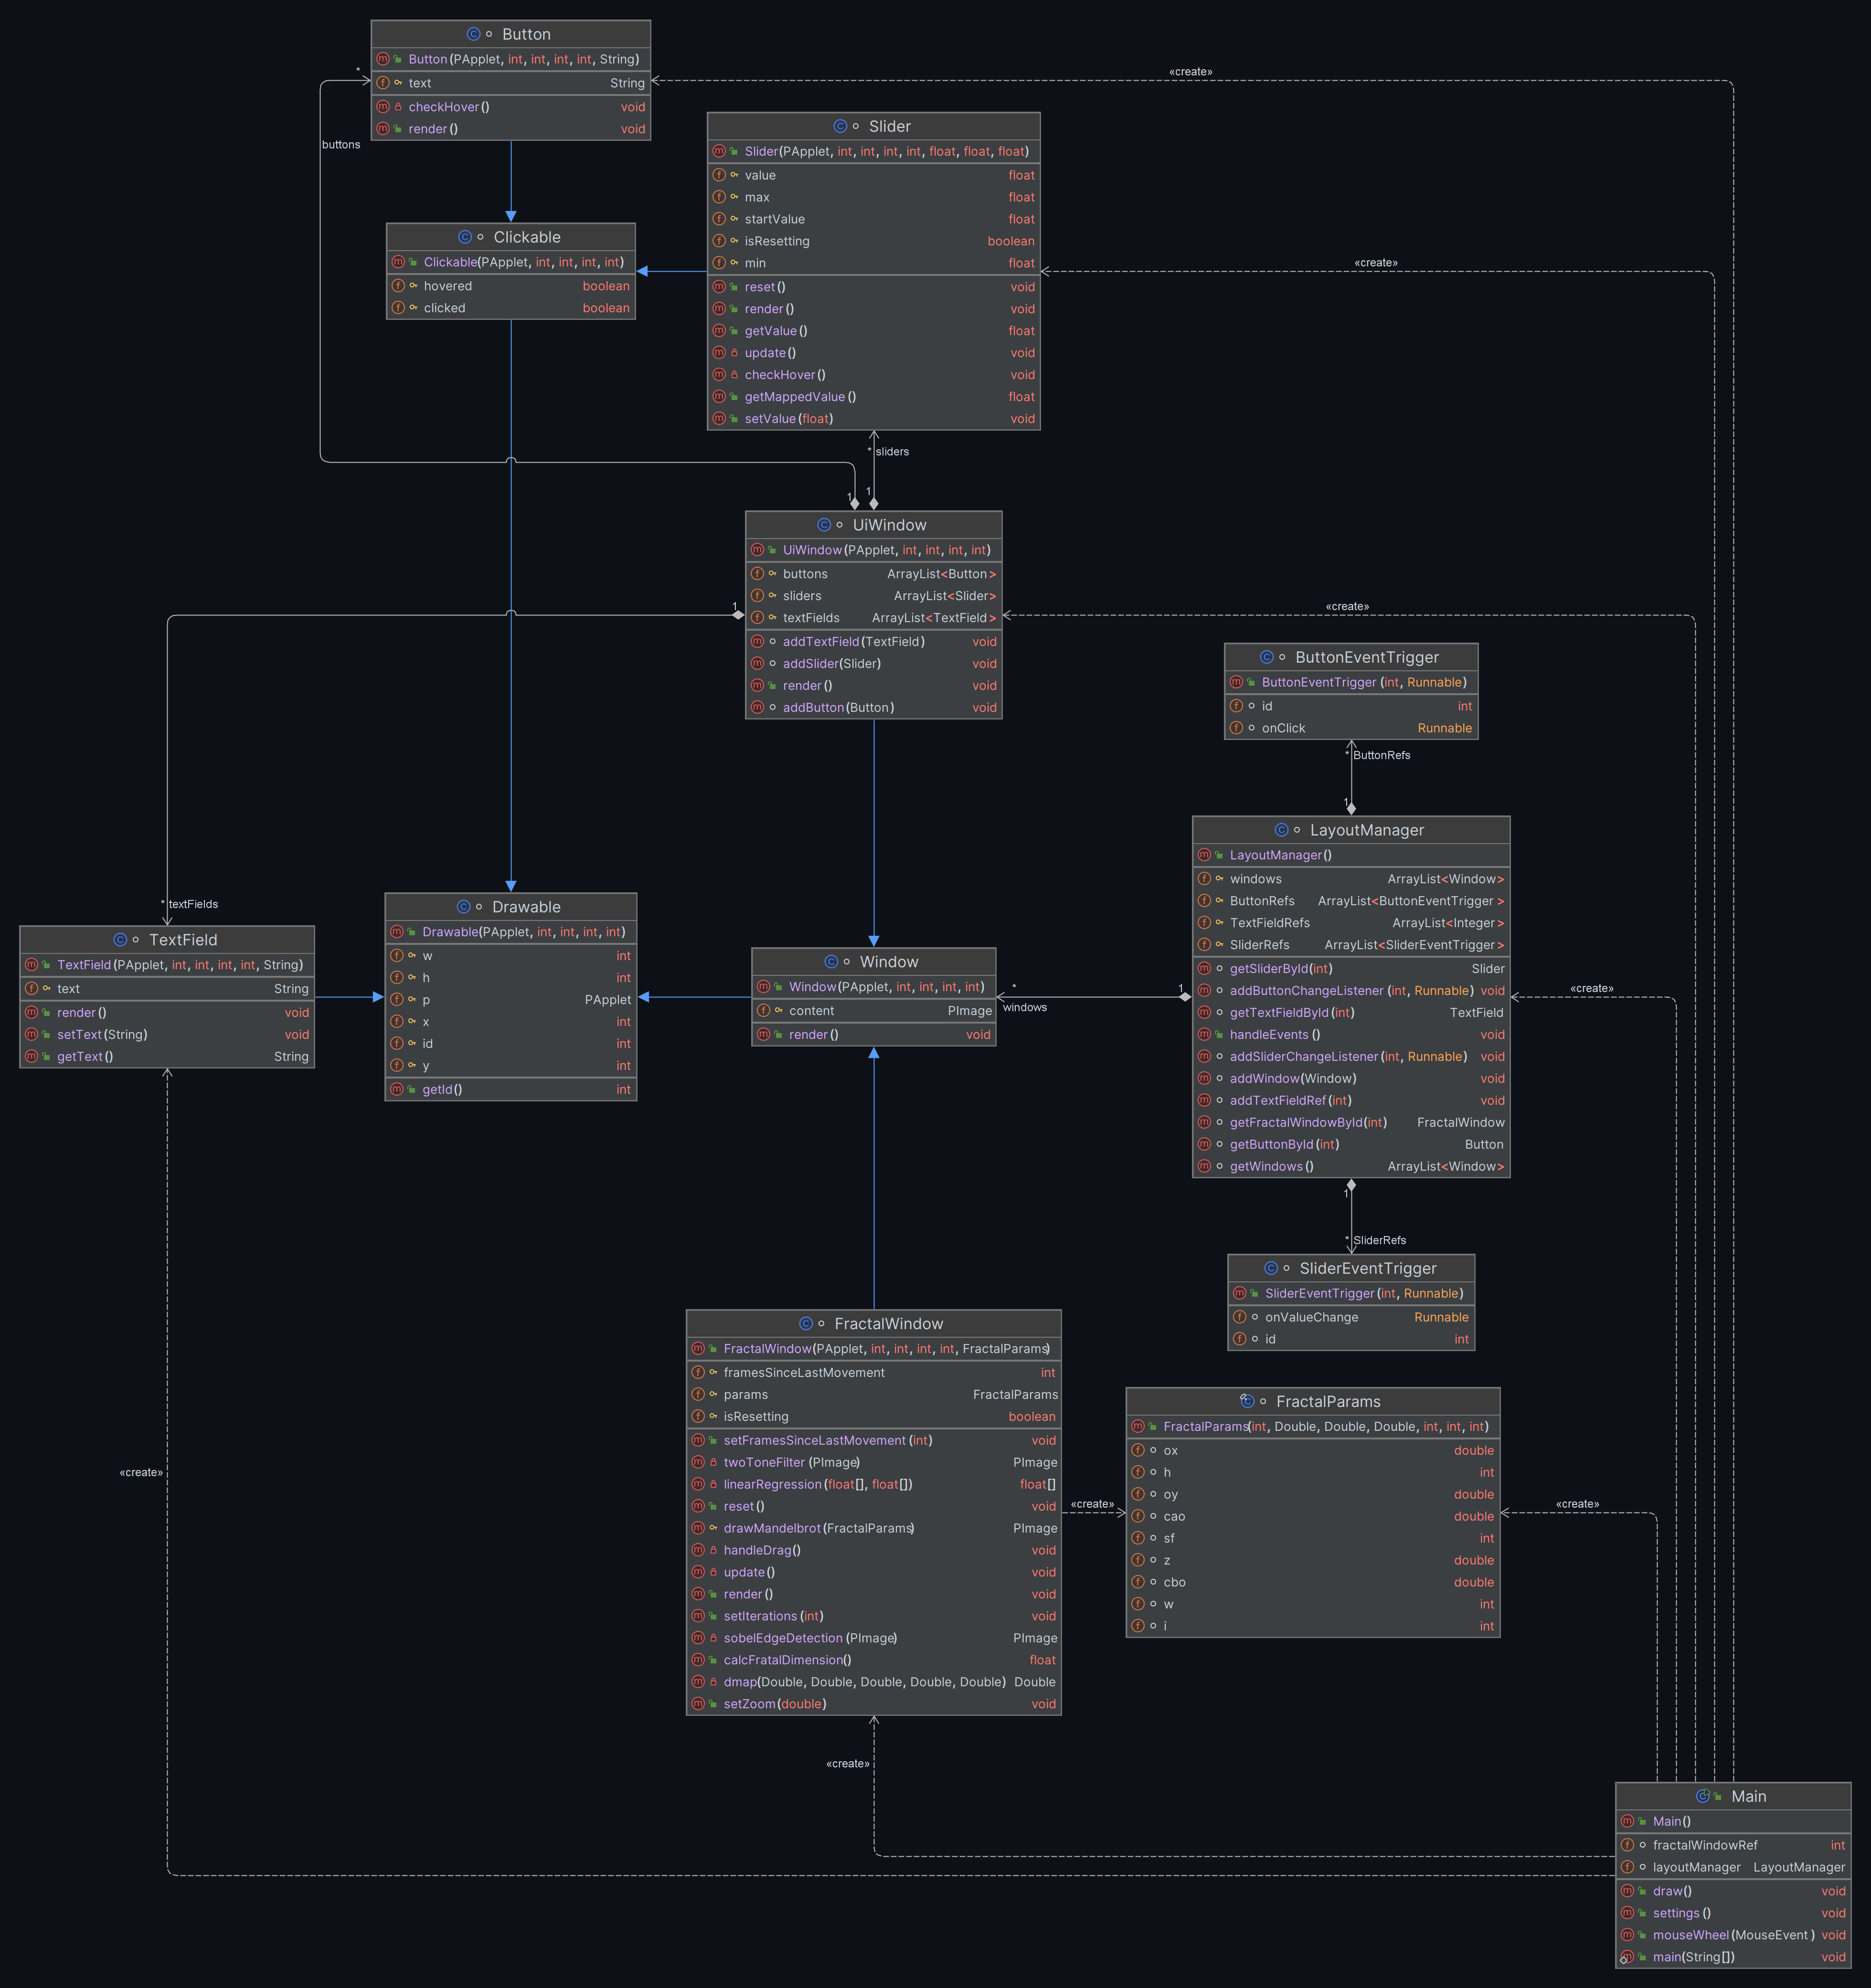
\includegraphics[width=1\linewidth]{Main.png}
    \caption{UML klasse diagram af koden}
    \label{fig:enter-label}
\end{figure}\\
For at overholde \textit{Single Responsibility Principle} Skal klasser som \texttt{Main} ikke styre specifikke ting men hellere stå for at køre programmet som helhed, såvel som opstart af programmet. Programmet er opbygget af vinduer administreret af en \texttt{LayoutManager} som har til ansvar at holde og vinduerne i programmet og håndtere kommunikation mellem vinduerne. Ethvert \texttt{Drawable}, som er programmet mest abstrakte basisklasse, har et \texttt{id} som bruges som reference når et element skal kommuniere eller kalde en funktion i et andet element sikker og uden at bryde OOP principperne. For at gøre dette indeholder \texttt{LayoutManager} en slags kommunikations protokol til at håndtere knappernes og skydernes begivenheder og deres respektive handlinger. Først skal f.eks en knap konstrueres:
\begin{lstlisting}[language=Java]
Button resetButton = new Button(this, 50, 100, 100, 50, "Reset");
\end{lstlisting}
Da \texttt{Button} arver fra \texttt{Clickable} som arver fra \texttt{Drawable} skal parametrene \texttt{PApplet}, \texttt{x}, \texttt{y}, \texttt{w}, \texttt{h}, \texttt{text} defineres. Når objeket er lavet skal id'et gemmes i en lokal variabel til senere brug:
\begin{lstlisting}[language=Java]
int resetButtonRef = resetButton.getId();
\end{lstlisting}
Nu kan knappen tilføjes til vinduet så den kan blive tegnet på skærmen:
\begin{lstlisting}[language=Java]
uiWindow.addButton(resetButton);
layoutManager.addWindow(uiWindow);
\end{lstlisting}
Nu skal \texttt{LayoutManager} vide hvad der skal ske når knappen trykkes, denne aktion kan udtrykkes som en lambda-funktion (en ikke navngivet funktion) som bruges som argument i en \texttt{changeListener}:
\begin{lstlisting}[language=Java]
layoutManager.addButtonChangeListener(
        resetButtonRef,
        () -> {
            Button el = layoutManager.getButtonById(resetButtonRef);
            FractalWindow fractal = layoutManager.getFractalWindowById(fractalWindowRef);
            Slider caoSliderEl = layoutManager.getSliderById(caoSliderRef);
            Slider cboSliderEl = layoutManager.getSliderById(cboSliderRef);
            if (el instanceof Button && fractal instanceof FractalWindow) {
                ((Button) el).clicked = false;
                fractal.reset();
                caoSliderEl.reset();
                cboSliderEl.reset();
            }
        });
\end{lstlisting}
På den måde holdes funktionaliteten inde i \texttt{LayoutManager} klassen som har til formål at tillade kommunikation mellem elementer. Samme tilgang bruges til de andre interaktive elementer i programmet. Programmet overholder også \textit{Liskov Substitution Principle} idet f.eks klassen \texttt{Clickable} kunne erstatte klassen \texttt{Drawable} idet funktionaliteten er bevaret (i dette tilfælde uden overhovedet at overskrive). Programmet overholder også indkapslings princippet idet der ikke er direkte adgang til variablerne f.eks. i \texttt{LayoutManager} klassen er de interne reference \texttt{ArrayList<...>} ikke tilgængelige, men klassen tilbyder metoder til at tilføje og finde et element, dette gør den endelige kode bedre, mere sikker og mere læsbar.
\section{Minkowski–Bouligand dimension i praksis}
\begin{wrapfigure}{r}{6cm}
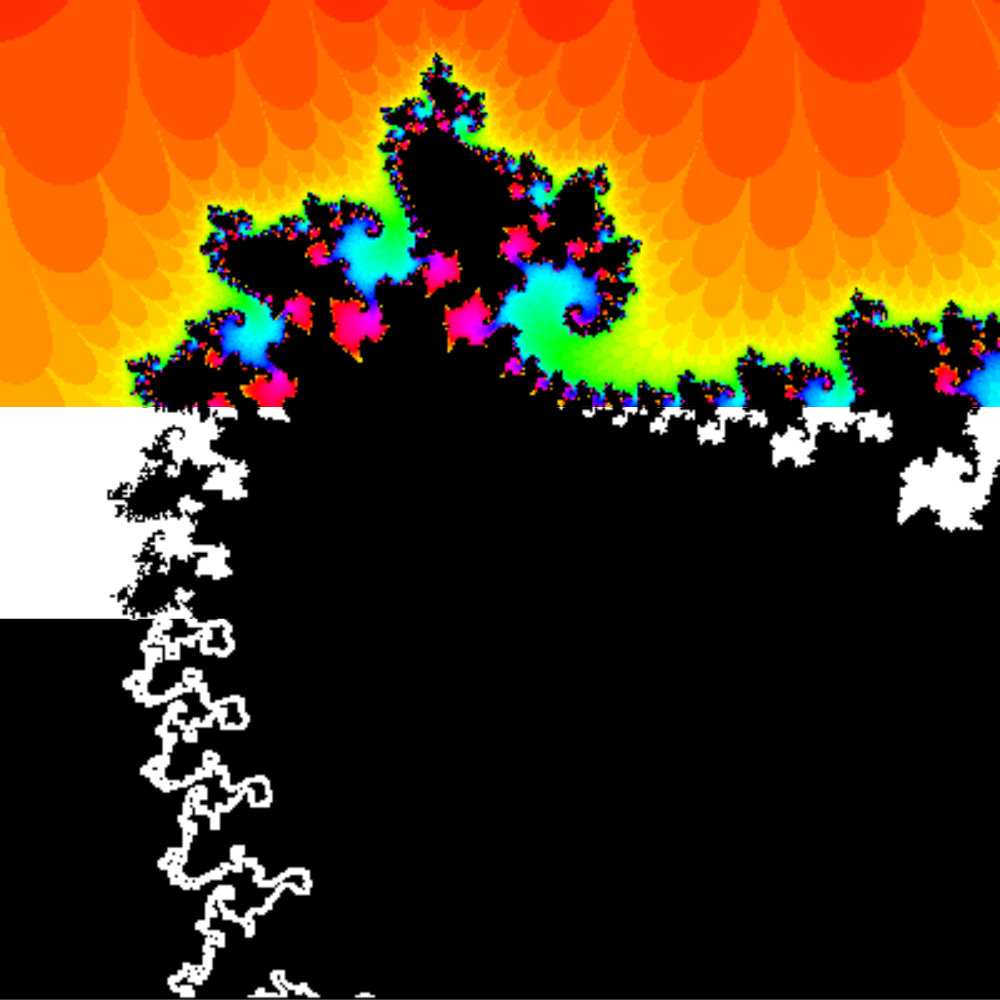
\includegraphics[width=6cm]{dimansion.png}
\caption{Billede processering til box-counting}\label{wrap-fig:idk}
\end{wrapfigure}
Formlen for Minkowski–Bouligand dimension: $$D = \lim_{\epsilon\to0} \frac{\log(\text{N}(\epsilon)}{\log(\frac{1}{\epsilon})}$$ ikke giver mening i praksis, da vores boksstørrelse skal tilnærme sig 0 og derfor vil udregningen tage uendelig lang tid. vi bliver altså også har nåd til at lave en tilnærmelse, ligesom alt andet i "fraktal-land". Dette gøres ved brug af lineær regression. i denne regression defineres et koordinat system hvor x-aksen er lig $\log(\frac{1}{\epsilon})$ og y-aksen er lig $\log(\text{N}(\epsilon)$. i dette tilfælde er $\epsilon$ lig nedskaleringsfaktoren af billedet så: $\frac{\text{startBilledstørrelse}}{\text{nedskaleringsfaktoren}}=\text{billedstørrelse}$ og $\text{N}(\epsilon)$ er mægnden af hvide pixels i billedet. Men vi kan ikke bruge det oprindelige billed da formlen kun virker med kanten af fraktalen, af den grund skal fraktal billedet gennem en billede processerings algoritme, på billedt til højdre ses de 2 skridt i denne process, først skal alt hvad der ikke er sort sættet til hvidt, derefter skal der køres en edge detection algoritme på billedet, nu kan de hvide pixels optælles og derefter kan en lineær regression udføres hvor hældningskoefficienten er ca. lig $D$. Herunder analyseres programmets implementation at de 2 lag i programmets billede processerings algoritme samt programmets implementation at lineær regression.
\newpage
\subsection{Sort-hvid filter}
\lstinputlisting[language=Java]{twotone.java}
Denne simple algoritme kigger på hver pixel og erstatter hver pixel som ikke er sort med hvid, da \texttt{pixels[]} ikke er et 2 dimensionalt liste i Processing skal y værdigen ganges med bredden af billedet. denne funktion er en del af \texttt{FractalWindow} klassen.\\\\
\subsection{Sobel-kantdetektion}
\lstinputlisting[language=Java]{sobel.java}
Sobel-kantdetektion er en algoritme, der finder kanter i et billede ved at beregne gradientet for hver pixel. Den bruger to separate filtreringskerner, en for horisontal gradient (\texttt{gx}) og en for vertikal gradient (\texttt{gy}), til at udregne ændringen i intensitet i x- og y-retningen for hver pixel. For hver pixel i billedet, undtagen den yderste kant, beregnes værdierne for de omkringliggende pixels ved hjælp af en 3x3 maske, og disse bruges til at beregne det horisontale og vertikale gradient. Derefter findes den samlede gradient ved at tage kvadratroden af summen af kvadraterne af \texttt{gx} og \texttt{gy}, og denne værdi opdateres i det resulterende billede. Højere gradientværdier indikerer stærkere kanter, hvilket gør det muligt at identificere kanter i originalbilledet. Siden billedet har været igennem et sort-hvid filter på det tidspunkt vil det resulterende gradient næsten altid være perfekt hvid.
\newpage
\subsection{Lineær regression}
\lstinputlisting[language=Java]{linear.java}
Denne kode beregner koefficienterne \( a \) og \( b \) for en lineær regressionsmodel ved hjælp af mindste kvadraters metode. Den itererer over to lister \( x \) og \( y \), der indeholder henholdsvis de uafhængige og afhængige variable. Inden for løkken akkumuleres summer, der er nødvendige for beregning af \( a \) og \( b \), såsom summen af \( x \), \( y \), \( xy \) og \( x^2 \). Efter løkken beregner den \( a \) og \( b \) ved hjælp af formler, der er afledt fra mindste kvadraters metode, hvor \( a \) repræsenterer hældningen af regressionslinjen og \( b \) repræsenterer skæringspunktet med y-aksen. Metoden returnerer et liste indeholdende \( a \) og \( b \), som er koefficienterne for den lineære regressionsmodel. Denne kode er baseret på princippet om, at i en lineær regressionsmodel minimerer den bedst egnede linje summen af kvadraterne af de lodrette afstande mellem de observerede og forudsagte værdier.\\\\
\subsubsection{BEVIS for $a$ og $b$ i mindste kvadraters metode}
%For en lineær model \( y = ax + b \), hvor \( a \) er hældningen og \( b \) er skæringspunktet med y-aksen, kan vi definere en funktion, der repræsenterer den kvadrerede afstand mellem et punktsæt (krvadratsummen) hvor 1 punkt ser således ud: \((x_i, y_i)\) 
Residualet for et givet punkt \((x_i, y_i)\) i en lineær model \( y = ax + b \) , hvor \( a \) er hældningen og \( b \) er skæringspunktet med y-aksen, er lig:
$$
r_i=y_i-ax_i-b
$$
Så vil kvadratsummen af alle punkter være lig:
$$
K(a, b) = \sum_{i=1}^{n} r_i^2=\sum_{i=1}^{n} (y_i-ax_i-b)^2
$$
Nu differentieres $K$ med hensyn til både $a$ og $b$ og sættes til 0:\\
Lad os starte med $K'_b$ 
\begin{align*}
0&=K'_b(a,b)\\
0&=\sum_{i=1}^{n} 2(y_i-ax_i-b)(-1)                     &&\Leftrightarrow &&&\text{Differentieret med hensyn til $b$} \\
0&=-2\sum_{i=1}^{n} (y_i-ax_i-b)                        &&\Leftrightarrow &&&\text{sætter 2 og -1 ud foran} \\
0&=\sum_{i=1}^{n} (y_i-ax_i-b)                          &&\Leftrightarrow &&&\text{Da $K'_b=0$ kan $-2$ forkortes}\\
0&=\sum_{i=1}^{n}y_i-a\sum_{i=1}^{n}x_i-\sum_{i=1}^{n}b &&\Leftrightarrow &&&\text{Da det er tilladt at splitte summen op:}\\
0&=\sum_{i=1}^{n}y_i-a\sum_{i=1}^{n}x_i-nb              &&\Leftrightarrow &&&\text{Da $b$ er konstant}\\
nb&=\sum_{i=1}^{n}y_i-a\sum_{i=1}^{n}x_i                &&\Leftrightarrow &&&\text{plus $n\cdot b$ på bægge sider}\\
b&=\Bar{y}-a\Bar{x}                                     &&\Leftrightarrow &&&\text{divider med $n$ på begge sider, summene bliver til gennemsnit}\\
\end{align*}
Lad os nu udregne $K'_a$
\begin{align*}
0&=K'_a(a,b)\\
0&=\sum_{i=1}^{n}2(y_i-ax_i-b) (-x_i)                                      &&\Leftrightarrow &&&\text{Differentieret med hensyn til $a$} \\
0&=-2\sum_{i=1}^{n}x_i(y_i-ax_i-b)                                         &&\Leftrightarrow &&&\text{$2$ bliver til $-2$ da vi rykker 2 og $-x_i$ ud} \\
0&=\sum_{i=1}^{n}x_i(y_i-ax_i-b)                                           &&\Leftrightarrow &&&\text{Da $K'_a=0$ kan $-2$ forkortes}\\
0&=\sum_{i=1}^{n}x_i(y_i-ax_i-\Bar{y}+a\Bar{x})                            &&\Leftrightarrow &&&\text{Da $b = \Bar{y}-a\Bar{x}$}\\
0&=\sum_{i=1}^{n}x_i(y_i-\Bar{y})-a\sum_{i=1}^{n}x_i(x_i-\Bar{x})          &&\Leftrightarrow &&&\text{Jeg splitter parentesen i y og x dele}\\
a\sum_{i=1}^{n}x_i(x_i-\Bar{x})&=\sum_{i=1}^{n}x_i(y_i-\Bar{y})            &&\Leftrightarrow &&&\text{Plus $a\sum_{i=1}^{n}x_i(x_i-\Bar{x})$ på begge sider}\\
a&= \frac{\sum_{i=1}^{n}x_i(y_i-\Bar{y})}{\sum_{i=1}^{n}x_i(x_i-\Bar{x})}  &&\Leftrightarrow &&&\text{Divider $\sum_{i=1}^{n}x_i(x_i-\Bar{x})$ på begge sider}\\
\end{align*}
Nu er løsningen af $a$ og $b$ i mindste kvadraters metode bevist
\hfill\blacksquare
\section{Forbedringsforslag}
Øget nøjagtighed i programmet vil øge programmets funktionalitet fordi selv med datatypen \texttt{double} løber man hurtig ind i begrænsninger da zoom funktionaliteten ikke er lineær. Øget nøjagtighed vil også øge præcisionen af dimension udregningerne. Dog vil udregninger ved en eventuel øget nøjagtighed også øge tiden det vil tage at udregne en opdatering, det er altså en balance mellem tid og nøjagtighed. Det vurderes at programmet har slået en god balance idet man aldrig skal vente, det hele køre i reeltid ihvertfald på en moderat kraftig laptop. Et andet område hvor programmets kunne forbedres er mængden af fraktaler man kan udforske og beregne fraktal dimension på, f.eks. kunne nogle at de mere simple fraktaler fra første afsnit inddrages og visualiseres. Men dette vurderes alligevel til at være udenfor opgaves krav. Programmets brugervenlighed vurderes til at være meget høj idet alt kan betjenes med musen direkte fra brugerfladen.
\section{Kystlinjer}
Lidt ligesom fraktaler har kystlinjer også den egenskab at de har uendelig detalje. Hvis du kigger med en detalje på 1 meter vil du få en anden længde end hvis du kigger ned til 1 millimeter detalje, på denne måde kan vi også her bruge box-counting til at tilnærme en fraktal dimension. f.eks. er kystlinjen af Norges lig ca. 1,31. \parencite{article} Men uanset hvor langt du zoomer ind vil der altid være mere detalje, dog vil du i den virkelige verden være begrenset af atomer, bøjer og mange andre ting.
\section{Opsamling}
Opgavens problemformulering lød således: \textit{Hvordan kan fraktaler anvendes i programmering og matematik, og hvordan kan forståelsen af disse komplekse systemer øges ved hjælp af visuelle værktøjer} For at løse denne problemformulering blev der lavet et visuelt udforsknings værktøj af mandelbrotmængden i reeltid, der har til formål at øge forståelsen af disse komplekse matematiske fænomener. Der blev også udforsket og implementeret en måde at udregne fraktal dimension af mandelbrotmængden ved at kigge på forskellige størrelser af billeder. Mens der naturligvis er plads til forbedring så er programmet bøde funktionelt og intuitivt som det er nu.
\newpage
\printbibliography
\newpage
\section{Bilag}
\subsection{Programmet}
\begin{figure}[!h]
    \centering
    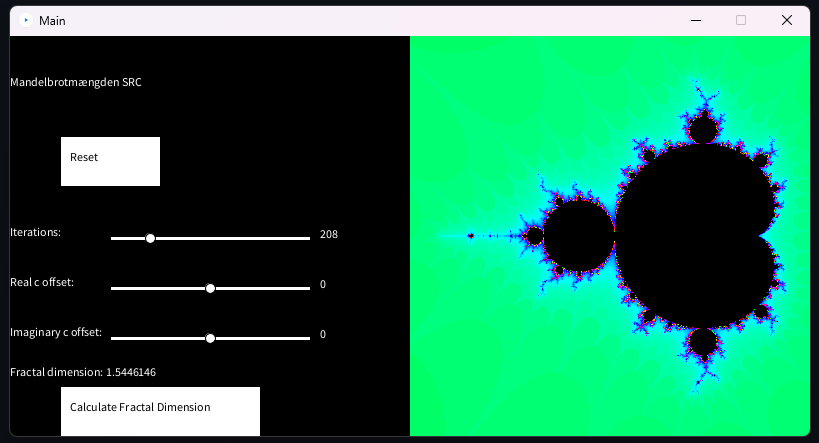
\includegraphics[width=1\linewidth]{program.png}
    \caption{Det færdige program}
    \label{fig:enter-label}
\end{figure}
\subsection{Kilde koden}
\href{https://github.com/victorDigital/SRC}
\end{document} 